\chapter{Data and Simulation Samples}
\label{chatper:data_and_mc_samples}

\section{Data}

The data used in this analysis were collected by the CMS detector in 2012 at a
center of mass energy of \rootseight. The LHC delivered 23 \fbinv of integrated
luminosity during the year as seen in \FIG~\ref{fig:2012_luminosity}. This
period was divided into four run eras called 2012A, B, C, and D. During an era,
the LHC run parameters are kept roughly static to allow for consistent data
taking conditions. In between eras, maintenance and minor upgrades were
performed on the LHC in order to deliver higher luminosity.

\begin{figure}[!htbp]
    \centering
    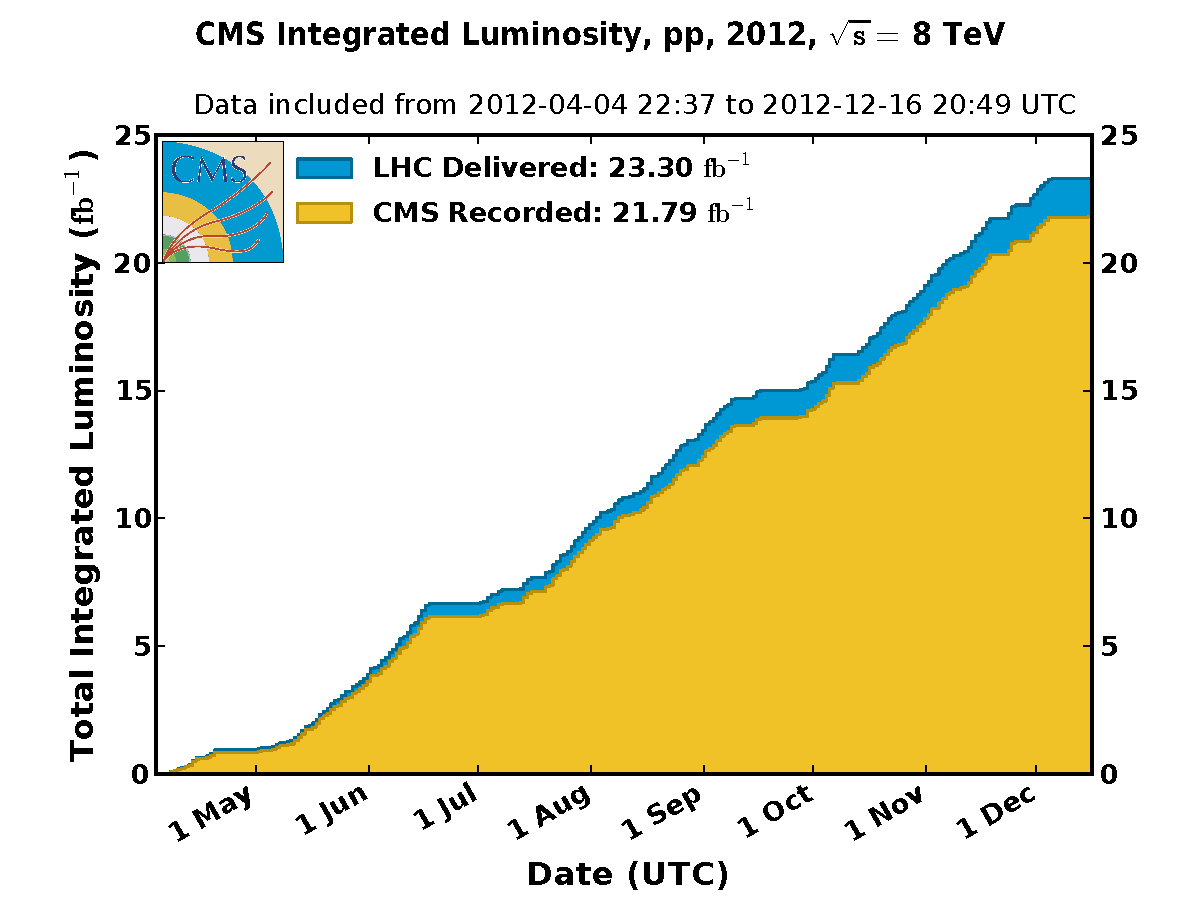
\includegraphics[width=\textwidth]{figures/2012_lumi.pdf}
    \caption{The integrate luminosity per day delivered and recorded by CMS in
        2012. The flat periods in May, July, and September correspond to the
        boundaries between the run eras.}
    \label{fig:2012_luminosity}
\end{figure}

The data collected by CMS are split into smaller datasets based on the physics
objects contained within the events. This allows analyses to use only one or
two datasets, instead of requiring them to deal with the entirety of the CMS
data (which is petabyte scale, and hence too large for most institutes to store
locally). The HLT sorts events into the various datasets based on the triggers
that the event fired. In this manner, an event can end up in multiple datasets
if it fired multiple triggers. This analysis uses the \SingleElectron dataset
which was collected with the HLT trigger \SingleElectronTrigger. These datasets
were reconstructed---converted from raw detector response into physics
objects---in January, 2013, in order to make use of the most recent
calibrations derived from the entire 2012 run. A summary of the datasets used
are listed in \TAB~\ref{table:datasets}.

\begin{table}[h]
\centering
\begin{center}
    \begin{tabular}{ | l | c | c |}
    \hline
    Dataset Name                          & Run Dates                & Luminosity       \\ \hline
    /SingleElectron/Run2012A-22Jan2013-v1 & 2012-04-05 to 2012-05-08 & $889.362 \pbinv$ \\ \hline
    /SingleElectron/Run2012B-22Jan2013-v1 & 2012-05-10 to 2012-06-18 & $4.429 \fbinv$   \\ \hline
    /SingleElectron/Run2012C-22Jan2013-v1 & 2012-07-01 to 2012-09-27 & $7.152 \fbinv$   \\ \hline
    /SingleElectron/Run2012D-22Jan2013-v1 & 2012-09-28 to 2012-12-06 & $7.318 \fbinv$   \\ \hline
    \end{tabular}
\end{center}
\caption{
    The datasets used in this analysis.
}
\label{table:datasets}
\end{table}

Although there is a \DoubleElectron dataset which uses a trigger designed to
find Z bosons, this analysis uses the \SingleElectron dataset selected with the
\SingleElectronTrigger trigger. The primary motivation behind using this
trigger was to allow a direct comparison with a similar \phistar analysis being
performed by CMS which used \Ztomumu events selected with a single muon
trigger. The single electron trigger requires an electron with $\pt > 27$ which
passes Working Point 80 (\WPEighty), a set of selection requirements on lepton
isolation and shower shape designed to be 80\% efficient in selecting real
electrons. The requirements that make up \WPEighty are listed in
\TAB~\ref{table:wp80}. This trigger had the lowest \pt threshold of any single
electron trigger that was unprescaled run during 2012. To prescale a trigger
means to apply a rate reduction by randomly throwing out a certain fraction of
events in order to keep the total trigger rate manageable; as this trigger was
unprescaled, no events were discarded in this manner.

\begin{table}[h]
\centering
\begin{center}
    \begin{tabular}{ | c | c c |} \hline
        Value                      & EB     & EE     \\ \hline
        $|\eta| <$                 & 1.4791 & 2.65   \\
        $\pt >$                    & 27     & 27     \\
        $\sigmaietaieta <$         & 0.1    & 0.03   \\
        $\ECALISO / \et <$         & 0.15   & 0.1    \\
        $\HOverE <$                & 0.1    & 0.05   \\
        $\HCALISO / \et <$         & 0.1    & 0.1    \\
        Pixel Matching $\ge$       & 1      & 1      \\
        $|\ooeoop| <$              & 0.05   & 0.05   \\
        $|\Delta \eta| <$          & 0.007  & 0.007  \\
        $|\Delta \phi| <$          & 0.06   & 0.03   \\ \hline
    \end{tabular}
\end{center}
\caption{
    The selection requirements for the \SingleElectronTrigger trigger for
    electrons which end up in the barrel region or the endcap region of ECAL.
    The variables used are detailed in \SEC~\ref{sec:electron_variables}.
}
\label{table:wp80}
\end{table}

The events from the \SingleElectron sample are further filtered for quality. A
centrally produced list of good luminosity segments is used to select only
events in which no part of the detector was malfunctioning or disabled. After
accounting for detector dead time and beam quality, \GoodLumiNumber of
integrated luminosity are used for physics analysis.

\section{Monte Carlo Datasets}
\label{ssec:monte_carlo}

This analysis makes use of numerous simulated data samples---colloquially
referred to as Monte Carlo (MC)---in order to estimate backgrounds and signal
yields, derive scale factors, and correct for the effects of bin migration on
the final measurement. All the MC used in this analysis were central generated
by the CMS collaboration. A \DYtoll signal sample and a $\ttbar\text{+jets}$
background sample were generated with \MADGRAPH \cite{alwall2014}. Diboson
($\Z\Z$, $\W\Z$, $\W\W$) background samples and a \DYtotautau background sample
were generated with \PYTHIA \cite{sjostran2006}. Background samples consisting
of $\tbar \W$, $t \W$, and $\DYtotautau$ were generated using \POWHEG
\cite{nason2004}\cite{alioli2010}\cite{re2011}. A secondary signal MC was also
generated with \POWHEG. The details of these samples are listed in
\TAB~\ref{table:mc}.

\begin{table}[h]
\centering
\begin{center}
    \begin{tabular}{ | l | l c c |}
    \hline
    Process                                &  Generator & $\sigma$, pb  & Events $(\times 10^{6})$ \\ \hline
    \DYtoll                                &  \MADGRAPH & 3531.9 (NNLO) & 30.460 \\
    \DYtoee                                &  \POWHEG   & 1966.7 (\TODO{??}) & 3.297\\
    \DYtotautau                            &  \POWHEG   & 1966.7 (\TODO{??})       & 3.297  \\
    \ttbar                                 &  \MADGRAPH & 23.64         & 3.984  \\
    $t \rightarrow \W+b \rightarrow X$     &  \POWHEG   & 11.1          & 0.498  \\
    $\tbar \rightarrow \W+b \rightarrow X$ &  \POWHEG   & 11.1          & 0.493  \\
    $\W\W$                                 &  \PYTHIA   & 54.84         & 10.000 \\
    $\W\Z$                                 &  \PYTHIA   & 33.21         & 10.000 \\
    $\Z\Z$                                 &  \PYTHIA   & 17.7          & 9.800  \\ \hline
    \end{tabular}
\end{center}
\caption{
    Summary of the MC samples used in this analysis. All cross sections are NLO
    unless otherwise stated. \TODO{Is POWHEG NLO?}
}
\label{table:mc}
\end{table}

After the generation step, MC is sent through a full detector simulation which
uses \GEANTfour \cite{agostinelli2003} to mimic the detector response. This
detector response is reconstructed using the full CMS reconstruction chain to
produce MC files that are in a format identical to actual data.

MC events have actual data events overlaid on top of them to better match the
conditions found in actual running. These overlaid events come from the minimum
bias dataset, which is selected with a minimum of requirements imposed on the
event in order to select events that are ``typical'' of proton-proton
collisions. Additional events are overlaid in order to simulate pileup. The
number of pileup events overlaid is drawn from a distribution that is expected
to match the distribution seen in data. Of course, it is not possible to
perfectly predict the data distribution and so a reweighting technique is used
to match the MC distribution to the data. The distribution in MC is compared to
that in data and the ratio of these distributions is assigned as a weight to
each MC event to force the distributions to match.

\section{Scale Factors}
\label{sec:scale_factors}

The detector response to various signals is not always perfectly simulated in
MC and so the efficiencies of various selection requirements are not the same
in data and MC. In order to correct this, each event in MC is reweighed with a
series of scale factors (SF) which are the efficiency of some selection process
in data divided by the same efficiency as measured on MC:

\begin{equation}
    \label{eq:sf}
    \text{SF} = \frac{\effdata}{\effmc}
\end{equation}

\subsection{Tag and Probe}

Tag and Probe (\TnP) is a minimally biased method of calculating the efficiency
of some analysis process. \TnP takes advantage of the well known mass and
narrow width of the \Z boson to select a set of electrons for which very few
selection requirements have been applied. This is done by finding one
high-quality electron, the tag, and another minimally biased object, the probe,
that could be an electron. The invariant mass of these objects is computed and
if it is near the \Z mass peak, it is very likely that the probe is also an
electron. These probe electrons then have further selection requirements
applied to them, and the fraction that pass is taken as the efficiency of that
selection step.

\subsection{Electron Reconstruction}
\label{ssec:sf_reconstruction}

Electron reconstruction begins with the assembly of a supercluster in ECAL, and
ends with the matching of a supercluster to a track in the tracker. The details
of Electron reconstruction are described in
\SEC~\ref{sec:electron_reconstruction}. The efficiency of an electron with $\pt
> 20 \GeV$ depositing enough energy in ECAL to be reconstructed into a
supercluster is very high, although the exact efficiency must be measured in
MC as there is no more basic object with which to perform \TnP to measure it in
data. SF for matching a track given that a supercluster has already been found
were measured centrally by the CMS collaboration using \TnP
\cite{gsf_scale_factors_2013}.

The events used to measure the reconstruction SF are selected with the
dedicated electron \TnP Trigger: \TnPTrigger. This trigger requires one
electron with $\pt > 20 \GeV$ which must also pass very tight isolation and ID
requirements while requiring only a low energy ($\et > 4 \GeV$) supercluster as
the other leg. The trigger rate is kept down by requiring that the invariant
mass of these two objects is greater than $50 \GeV$.

These events are further required to pass a set of offline selection
requirements. The tag electron is required to pass \EGTIGHT, have $\pt > 25
\GeV$, and $|\eta| < 2.5$. Electrons are rejected if they fall in the seem
between EB and EE ($1.4442 < |\eta| < 1.566$). The tag must also be matched to
the tight leg of the \TnP trigger. The probe supercluster has minimal
requirements applied; it is required to have tracker isolation $< 0.15$. For
the MC sample, the tag is only required to be matched to a generator level
electron with $\Delta R < 0.2$. Additionally, the event was required to have
low \particleflow missing energy $\PFMET < 20 \GeV$. \TODO{Explain PF MET?}

The events were binned in terms of probe's $\pt$ and $\eta$ as well as whether
the probe passed or failed. In each bin the \mee distribution was constructed
and a template consisting of the sum of a Gaussian smeared \Ztoee MC sample and
an exponential background was fitted. The number of events predicted by the
signal fit on the passing sample, failing sample, and sum of the two samples
was used to get the efficiency. A similar process was performed on MC, although
instead of a fit a simple counting of passing events was performed (as there is
no background in MC). The resulting SF are given in
\TAB~\ref{table:gsf_scale_factor}.

\begin{table}[h]
\centering
\begin{center}
    \begin{tabular}{ | c | c | c | c | c |} \hline
	$|\eta|$                 & 20--30 \GeV                        & 30--40 \GeV                        & 40--50 \GeV                        & $>$ 50 \GeV                        \\ \hline
	\numrange{0.0}{0.8}      & $\effstatsys{0.982}{0.003}{0.012}$ & $\effstatsys{0.988}{0.001}{0.008}$ & $\effstatsys{0.990}{0.001}{0.004}$ & $\effstatsys{0.990}{0.001}{0.004}$ \\ \hline
	\numrange{0.8}{1.4442}   & $\effstatsys{0.993}{0.002}{0.012}$ & $\effstatsys{0.993}{0.001}{0.008}$ & $\effstatsys{0.993}{0.001}{0.004}$ & $\effstatsys{0.991}{0.001}{0.004}$ \\ \hline
	\numrange{1.4442}{1.566} & $\effstatsys{1.016}{0.012}{0.020}$ & $\effstatsys{0.985}{0.004}{0.009}$ & $\effstatsys{0.987}{0.004}{0.004}$ & $\effstatsys{0.974}{0.009}{0.006}$ \\ \hline
	\numrange{1.566}{2.0}    & $\effstatsys{0.988}{0.003}{0.012}$ & $\effstatsys{0.993}{0.002}{0.008}$ & $\effstatsys{0.992}{0.001}{0.004}$ & $\effstatsys{0.990}{0.003}{0.004}$ \\ \hline
	\numrange{2.0}{2.5}      & $\effstatsys{1.002}{0.004}{0.012}$ & $\effstatsys{1.004}{0.002}{0.008}$ & $\effstatsys{1.005}{0.002}{0.004}$ & $\effstatsys{0.998}{0.004}{0.004}$ \\ \hline
    \end{tabular}
\end{center}
\caption{
    Scale factors for GSF electron reconstruction. The upper uncertainty listed
    is statistical, the lower is systematic.
}
\label{table:gsf_scale_factor}
\end{table}

\subsection{Electron Identification}
\label{ssec:sf_id}

Not all electrons which are reconstructed pass the ID criteria used in this
analysis, specifically \EGMEDIUM and \EGTIGHT, the details of which are covered
in \SEC~\ref{ssec:electron_selection}. The efficiency of going from a
reconstructed electron to one which passes the identification criteria is
measured centrally by the CMS collaboration using \TnP \cite{cms_an_2014-055}.

The events used for this measurement were selected using two triggers: \\
\TnPTrigger, which is described above, and \TnPTriggerSecond, which requires
one electron with $\pt > 17 \GeV$ and tight isolation and ID requirements while
also requiring a reconstructed second electron (as opposed to a supercluster as
required by the first trigger) with $\pt > 8 \GeV$. It further requires a
dielectron invariant mass of $\mee > 50 \GeV$.

The tag electrons are required to pass \EGTIGHT, have $\pt > 25 \GeV$, and
$|\eta| < 2.5$; they are rejected if they fall in the seem between EB and EE
($1.4442 < |\eta| < 1.566$). The tag is not required to match the trigger.
Probe electrons have the same $\eta$ requirements as tags, but are only
required to have $\pt > 10 \GeV$. Passing probes pass the ID criteria under
investigation, failing probes fail the ID criteria. The invariant mass of the
tag and probe pair is required to be near the \Z mass peak (\MassRange). The
electrons are required to have charges of opposite sign. In MC, the probe is
only required to be matched to a generator electron with $\Delta R < 0.2$.

The efficiencies are then calculated by fitting the \mee distributions using a
template constructed with a \Ztoee MC sample and an exponential background. The
three categories (passing probes, failing probes, and all probes) are then
simultaneously fit with this template and the number of fitted signal events is
used to derive an efficiency. A simple count of events is used for the MC
efficiency instead of a fit. The resulting SF are given in
\TABS~\ref{table:tight_scale_factor} and \ref{table:medium_scale_factor}.

\begin{table}[h]
\centering
\begin{center}
    \begin{tabular}{ | c | c | c | c | c |} \hline
	$|\eta|$                 & 20--30 \GeV               & 30--40 \GeV               & 40--50 \GeV               & 50--200 \GeV \\ \hline
	\numrange{0.0}{0.8}      & $0.960_{-0.003}^{+0.003}$ & $0.978_{-0.001}^{+0.001}$ & $0.981_{-0.001}^{+0.001}$ & $0.982_{-0.002}^{+0.002}$ \\ \hline
	\numrange{0.8}{1.4442}   & $0.936_{-0.004}^{+0.004}$ & $0.958_{-0.002}^{+0.002}$ & $0.969_{-0.001}^{+0.001}$ & $0.969_{-0.002}^{+0.002}$ \\ \hline
	\numrange{1.4442}{1.566} & $0.933_{-0.017}^{+0.015}$ & $0.907_{-0.008}^{+0.008}$ & $0.904_{-0.004}^{+0.004}$ & $0.926_{-0.011}^{+0.011}$ \\ \hline
	\numrange{1.566}{2.0}    & $0.879_{-0.007}^{+0.007}$ & $0.909_{-0.003}^{+0.003}$ & $0.942_{-0.002}^{+0.002}$ & $0.957_{-0.004}^{+0.004}$ \\ \hline
	\numrange{2.0}{2.5}      & $0.974_{-0.004}^{+0.004}$ & $0.987_{-0.004}^{+0.004}$ & $0.991_{-0.003}^{+0.003}$ & $0.999_{-0.005}^{+0.005}$ \\ \hline
    \end{tabular}
\end{center}
\caption{
    Scale factors for \EGTIGHT electron ID.
}
\label{table:tight_scale_factor}
\end{table}

\begin{table}[h]
\centering
\begin{center}
    \begin{tabular}{ | c | c | c | c | c |} \hline
	$|\eta|$                 & 20--30 \GeV               & 30--40 \GeV               & 40--50 \GeV               & 50--200 \GeV \\ \hline
	\numrange{0.0}{0.8}      & $0.986_{-0.001}^{+0.002}$ & $1.002_{-0.001}^{+0.001}$ & $1.005_{-0.001}^{+0.001}$ & $1.004_{-0.001}^{+0.001}$ \\ \hline
	\numrange{0.8}{1.4442}   & $0.959_{-0.003}^{+0.003}$ & $0.980_{-0.001}^{+0.001}$ & $0.988_{-0.001}^{+0.001}$ & $0.988_{-0.002}^{+0.002}$ \\ \hline
	\numrange{1.4442}{1.566} & $0.967_{-0.013}^{+0.007}$ & $0.950_{-0.007}^{+0.006}$ & $0.958_{-0.005}^{+0.005}$ & $0.966_{-0.009}^{+0.009}$ \\ \hline
	\numrange{1.566}{2.0}    & $0.941_{-0.005}^{+0.005}$ & $0.967_{-0.003}^{+0.003}$ & $0.992_{-0.002}^{+0.002}$ & $1.000_{-0.003}^{+0.003}$ \\ \hline
	\numrange{2.0}{2.5}      & $1.020_{-0.003}^{+0.003}$ & $1.021_{-0.003}^{+0.003}$ & $1.019_{-0.002}^{+0.002}$ & $1.022_{-0.004}^{+0.004}$ \\ \hline
    \end{tabular}
\end{center}
\centering
\caption{
    Scale factors for \EGMEDIUM electron ID.
}
\label{table:medium_scale_factor}
\end{table}

\subsection{Single Electron Trigger}
\label{ssec:sf_trigger}

The efficiency of the HLT trigger used in this analysis,
\SingleElectronTrigger, is measured using \TnP on the primary dataset. The
efficiency is measured in bins of probe \pt and probe $\eta$ with bin
boundaries of \{30, 40, 50, 70, 250\} in \pt and \{-2.1, -2.0, -1.556, -1.442,
-0.8, 0., 0.8, 1.442, 1.556, 2.0, 2.1\} in $\eta$.

Both the tag electron and the probe electron are required to satisfy $|\eta| <
2.1$, $\pt > 30$, and to pass \EGTIGHT requirements. The pair must have an
invariant mass such that \MassRange. The tag electron is required to be matched
to an electron that fired the trigger with $\Delta R < 0.3$. There is no
requirement placed on the charge of the electron pair. Events with three or
more electrons are rejected.

Probes are considered passing if they are also matched to an electron that
fired the trigger with $\Delta R < 0.3$, and failing otherwise. The efficiency
in each bin is the number of passing probes divided by the number of failing
probes using a simple count. In an individual event, both electrons are tried
as a tag so that an event may contribute to the efficiency measurement twice if
both electrons pass the tag requirements.

The efficiency is computed in exactly the same way on the \MADGRAPH sample. The
MC events are reweighted for pileup, reconstruction efficiency, and
identification efficiency before the trigger efficiency is measured. The
measured efficiencies for data and MC are listed in
\TABS~\ref{trigger_eff_data} and \ref{trigger_eff_mc}, respectively.

In the case of the trigger, because either electron could cause the event to
pass, the SFs can not be computed for each bin, but instead must be computed
for each pair of bins. If only one electron in the event has $\pt > 30$ and
$|\eta| < 2.1$ than the SF is simply that given by \EQ~\ref{eq:sf}, but if both
electrons pass those requirements than either could have fired the trigger, and
the SF is given by:

\begin{equation} \label{eq:sf_double}
    \text{SF}_{1 \text{ or } 2}
    =
    \frac{
        1 - \left( 1 - \effdata_{0} \right) \left( 1 - \effdata_{1} \right)
    } {
        1 - \left( 1 - \effmc_{0} \right) \left( 1 - \effmc_{1} \right)
    }
\end{equation}

Where $\effdata_{0,1}$ is the efficiency as measured in data for the 0th and
1st electrons, and $\effmc_{0,1}$ is the efficiency as measured in MC.
\EQ~\ref{eq:sf_double} is just the probability that one or both of the
electrons fired the trigger divided by the same quantity in MC. This equation
assumes that the probability of one electron firing the trigger is uncorrelated
with the probability of the other electron firing the trigger.

% Data
\begin{table}[h]
\begin{center}
    \begin{tabular}{ | c | c | c | c | c | c |} \hline
	$\eta$ & 30---40 \GeV & 40---50 \GeV & 50---70 \GeV & 70---250 \GeV  \\ \hline
	\numrange{-2.1}{-2} & $0.741^{+0.003}_{-0.003}$ & $0.773^{+0.003}_{-0.003}$ & $0.780^{+0.005}_{-0.005}$ & $0.79^{+0.01}_{-0.01}$  \\ \hline
	\numrange{-2}{-1.556} & $0.734^{+0.001}_{-0.001}$ & $0.772^{+0.001}_{-0.001}$ & $0.786^{+0.002}_{-0.002}$ & $0.792^{+0.005}_{-0.005}$  \\ \hline
	\numrange{-1.556}{-1.442} & $0.725^{+0.003}_{-0.003}$ & $0.821^{+0.002}_{-0.002}$ & $0.809^{+0.004}_{-0.004}$ & $0.848^{+0.010}_{-0.010}$  \\ \hline
	\numrange{-1.442}{-0.8} & $0.8930^{+0.0005}_{-0.0005}$ & $0.9396^{+0.0003}_{-0.0004}$ & $0.9509^{+0.0006}_{-0.0006}$ & $0.966^{+0.001}_{-0.001}$  \\ \hline
	\numrange{-0.8}{0} & $0.9213^{+0.0004}_{-0.0004}$ & $0.9528^{+0.0002}_{-0.0002}$ & $0.9601^{+0.0004}_{-0.0004}$ & $0.9692^{+0.0010}_{-0.0010}$  \\ \hline
	\numrange{0}{0.8} & $0.9174^{+0.0004}_{-0.0004}$ & $0.9473^{+0.0003}_{-0.0003}$ & $0.9561^{+0.0004}_{-0.0004}$ & $0.963^{+0.001}_{-0.001}$  \\ \hline
	\numrange{0.8}{1.442} & $0.8964^{+0.0005}_{-0.0005}$ & $0.9424^{+0.0003}_{-0.0003}$ & $0.9533^{+0.0006}_{-0.0006}$ & $0.966^{+0.001}_{-0.001}$  \\ \hline
	\numrange{1.442}{1.556} & $0.714^{+0.003}_{-0.003}$ & $0.823^{+0.002}_{-0.002}$ & $0.827^{+0.004}_{-0.004}$ & $0.861^{+0.009}_{-0.010}$  \\ \hline
	\numrange{1.556}{2} & $0.758^{+0.001}_{-0.001}$ & $0.800^{+0.001}_{-0.001}$ & $0.811^{+0.002}_{-0.002}$ & $0.823^{+0.005}_{-0.005}$  \\ \hline
	\numrange{2}{2.1} & $0.764^{+0.003}_{-0.003}$ & $0.792^{+0.002}_{-0.002}$ & $0.797^{+0.005}_{-0.005}$ & $0.82^{+0.01}_{-0.01}$  \\ \hline
    \end{tabular}
\end{center}
\centering
\caption{
    Electron trigger efficiency in data.
}
\label{trigger_eff_data}
\end{table}

% MC
\begin{table}[h]
\begin{center}
    \begin{tabular}{ | c | c | c | c | c | c |} \hline
	$\eta$ & 30---40 \GeV & 40---50 \GeV & 50---70 \GeV & 70---250 \GeV  \\ \hline
	\numrange{-2.1}{-2} & $0.734^{+0.004}_{-0.004}$ & $0.769^{+0.004}_{-0.004}$ & $0.771^{+0.008}_{-0.008}$ & $0.76^{+0.02}_{-0.02}$  \\ \hline
	\numrange{-2}{-1.556} & $0.736^{+0.002}_{-0.002}$ & $0.768^{+0.002}_{-0.002}$ & $0.779^{+0.003}_{-0.003}$ & $0.789^{+0.008}_{-0.008}$  \\ \hline
	\numrange{-1.556}{-1.442} & $0.791^{+0.004}_{-0.004}$ & $0.847^{+0.003}_{-0.003}$ & $0.850^{+0.006}_{-0.006}$ & $0.87^{+0.01}_{-0.02}$  \\ \hline
	\numrange{-1.442}{-0.8} & $0.9395^{+0.0006}_{-0.0006}$ & $0.9612^{+0.0004}_{-0.0004}$ & $0.9690^{+0.0007}_{-0.0008}$ & $0.980^{+0.002}_{-0.002}$  \\ \hline
	\numrange{-0.8}{0} & $0.9469^{+0.0005}_{-0.0005}$ & $0.9670^{+0.0003}_{-0.0003}$ & $0.9745^{+0.0005}_{-0.0005}$ & $0.982^{+0.001}_{-0.001}$  \\ \hline
	\numrange{0}{0.8} & $0.9466^{+0.0005}_{-0.0005}$ & $0.9665^{+0.0003}_{-0.0003}$ & $0.9739^{+0.0005}_{-0.0006}$ & $0.982^{+0.001}_{-0.001}$  \\ \hline
	\numrange{0.8}{1.442} & $0.9364^{+0.0007}_{-0.0007}$ & $0.9597^{+0.0004}_{-0.0004}$ & $0.9668^{+0.0008}_{-0.0008}$ & $0.979^{+0.002}_{-0.002}$  \\ \hline
	\numrange{1.442}{1.556} & $0.779^{+0.004}_{-0.005}$ & $0.841^{+0.003}_{-0.003}$ & $0.842^{+0.006}_{-0.006}$ & $0.86^{+0.02}_{-0.02}$  \\ \hline
	\numrange{1.556}{2} & $0.749^{+0.002}_{-0.002}$ & $0.786^{+0.002}_{-0.002}$ & $0.798^{+0.003}_{-0.003}$ & $0.810^{+0.008}_{-0.008}$  \\ \hline
	\numrange{2}{2.1} & $0.737^{+0.004}_{-0.004}$ & $0.769^{+0.004}_{-0.004}$ & $0.779^{+0.007}_{-0.008}$ & $0.82^{+0.02}_{-0.02}$  \\ \hline
    \end{tabular}
\end{center}
\centering
\caption{
    Electron trigger efficiency in \MADGRAPH MC.
}
\label{trigger_eff_mc}
\end{table}

\section{Electron Dressing}
\label{sec:electron_dressing}

\begin{figure}[!htbp]
    \centering
    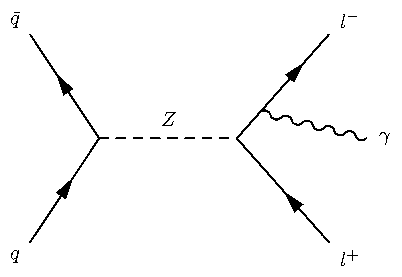
\includegraphics[width=0.65\textwidth]{figures/fsr.pdf}
    \caption{
        Feynman diagram of \Ztoll with FSR.
        % From http://www.physik.uzh.ch/~che/FeynDiag/ CC-BY-SA
    }
    \label{fig:fsr_diagram}
\end{figure}

After the \Ztoee decay, the electrons can radiate photons in a process known as
as final state radiation (FSR). This process is shown in
\FIG~\ref{fig:fsr_diagram}. This analysis defines three different types of
generator level electron in MC, each of which handles these photons slightly
differently. Each of these three definitions is then used whenever generator MC
is used in the analysis in order to produce three different final results. This
is done to make it easy to compare our results to theoretical models regardless
of how the models handle FSR. The three definitions of generator electrons are
as follows:

\begin{description}
    \item[Born] A generator electron immediately after the \Ztoee decay and
        before and FSR
    \item[Bare] A generator electron after it has shed all of its FSR photons
    \item[Dressed] A bare electron, but with its FSR photons added back in
        vector sum if they are within $\Delta R < 0.1$ of the electron
\end{description}

Generator level selection requirements are applied to dress electrons in this
analysis, for example, when selecting MC events to use for unfolding.
